
%(BEGIN_QUESTION)
% Copyright 2010, Tony R. Kuphaldt, released under the Creative Commons Attribution License (v 1.0)
% This means you may do almost anything with this work of mine, so long as you give me proper credit

Analyze this Allen-Bradley PLC program and explain what it is supposed to do:

$$\includegraphics[width=15.5cm]{i02377x01.eps}$$

\vfil

\underbar{file i02377}
\eject
%(END_QUESTION)





%(BEGIN_ANSWER)

This is a graded question -- no answers or hints given!

%(END_ANSWER)





%(BEGIN_NOTES)

The standard Start, Stop, and Seal-in contact structure in this program should remind you of every PLC-controlled motor system program you've ever seen.  The ``twist'' here is that there is an additional contact in series with the Stop contact, controlled by the ``Done'' bit on the counter instruction.  Being an NC virtual contact, it will force the ``Motor'' output bit to a 0 state whenever the counter reaches its preset count value.  

\vskip 10pt

Thus, the motor is inhibited from starting after 17 start/stop cycles.  This lockout counter may be reset by a discrete input ({\tt I:0/2}).

%INDEX% PLC, ladder logic program analysis and explanation

%(END_NOTES)



